\section{PTracking}

\begin{frame}
	\frametitle{Multi-Clustered Particle Filtering}
	
	\vspace{0.4cm}
	
	A \emph{Distributed Multi-Agent Multi-Object Tracking} method based on a \textbf{Multi-Clustered Particle
	Filter}.
	
	\vspace{0.3cm}
	
	\begin{itemize}
		\item \textbf{Input:} a set of positions of the objects provided by a Multi-Object detection system
		
		\vspace{0.4cm}
		
		\item \textbf{Output:} the estimated trajectories of the moving objects over time
	\end{itemize}
	
	\vspace{0.3cm}
	
	It is not a general solution yet...
	\vspace{-0.3cm}
	\begin{tabbing}
		\hspace*{0.3cm}
		$ \leadsto $ no target identity
	\end{tabbing}
\end{frame}

\begin{frame}
	\frametitle{Multi-Clustered Particle Filtering}
	\framesubtitle{Novelty}
	
	The novelties of the approach are:
	
	\vspace{0.3cm}
	
	\begin{itemize}
		\item a new clustering technique that keeps track of a variable unknown number of objects
		\vspace{0.2cm}
		\item an improved robustness and reduced network overload by using \emph{Gaussian Mixture Models}
		\vspace{0.2cm}
		\item an asynchronous approach to improve the flexibility and the robustness of the entire system
	\end{itemize}
\end{frame}

\begin{frame}
	\frametitle{Multi-Clustered Particle Filtering}
	\framesubtitle{Estimation Process}
	
	\vspace{0.3cm}
	
	\begin{center}
		\begin{tikzpicture}
			\node at (0,0) [draw=black,ultra thick,inner sep=0pt] {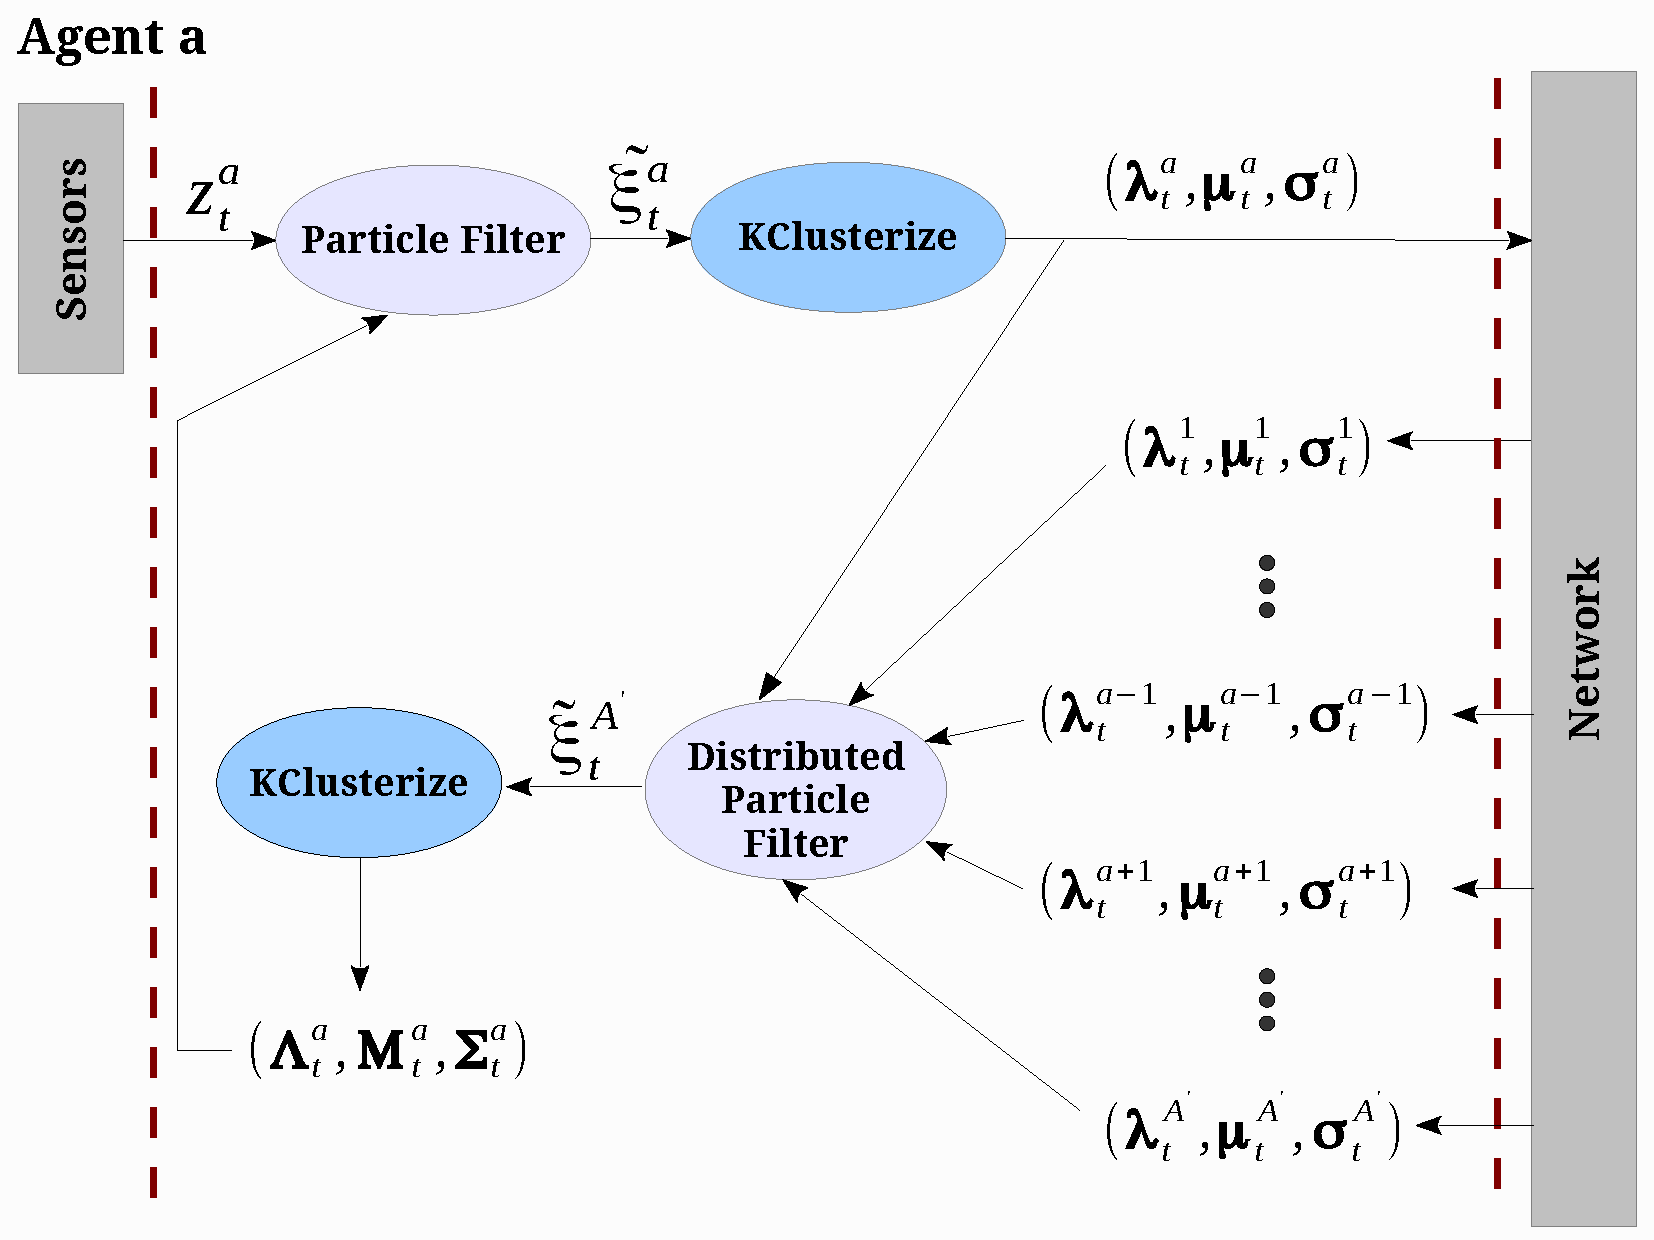
\includegraphics[scale=0.31]{images/EstProcess}};
		\end{tikzpicture}
	\end{center}
\end{frame}

\begin{frame}
	\frametitle{Experimental evaluation}
	\framesubtitle{Application field}
	
	\vspace{0.5cm}
	
	\emph{RoboCup Standard Platform League} using the \emph{Aldebaran Nao} humanoid robots and considering the task
	of tracking the ball in the soccer field.
	
	\vspace{0.3cm}
	
	The Multi-Clustered Particle Filter method is the core of the \emph{PTracking} software library used for the
	experimental evaluation.
	
	\vspace{0.2cm}
	
	\begin{center}
		\begin{tikzpicture}
			\node at (0,0) [draw=black,ultra thick,inner sep=0pt] {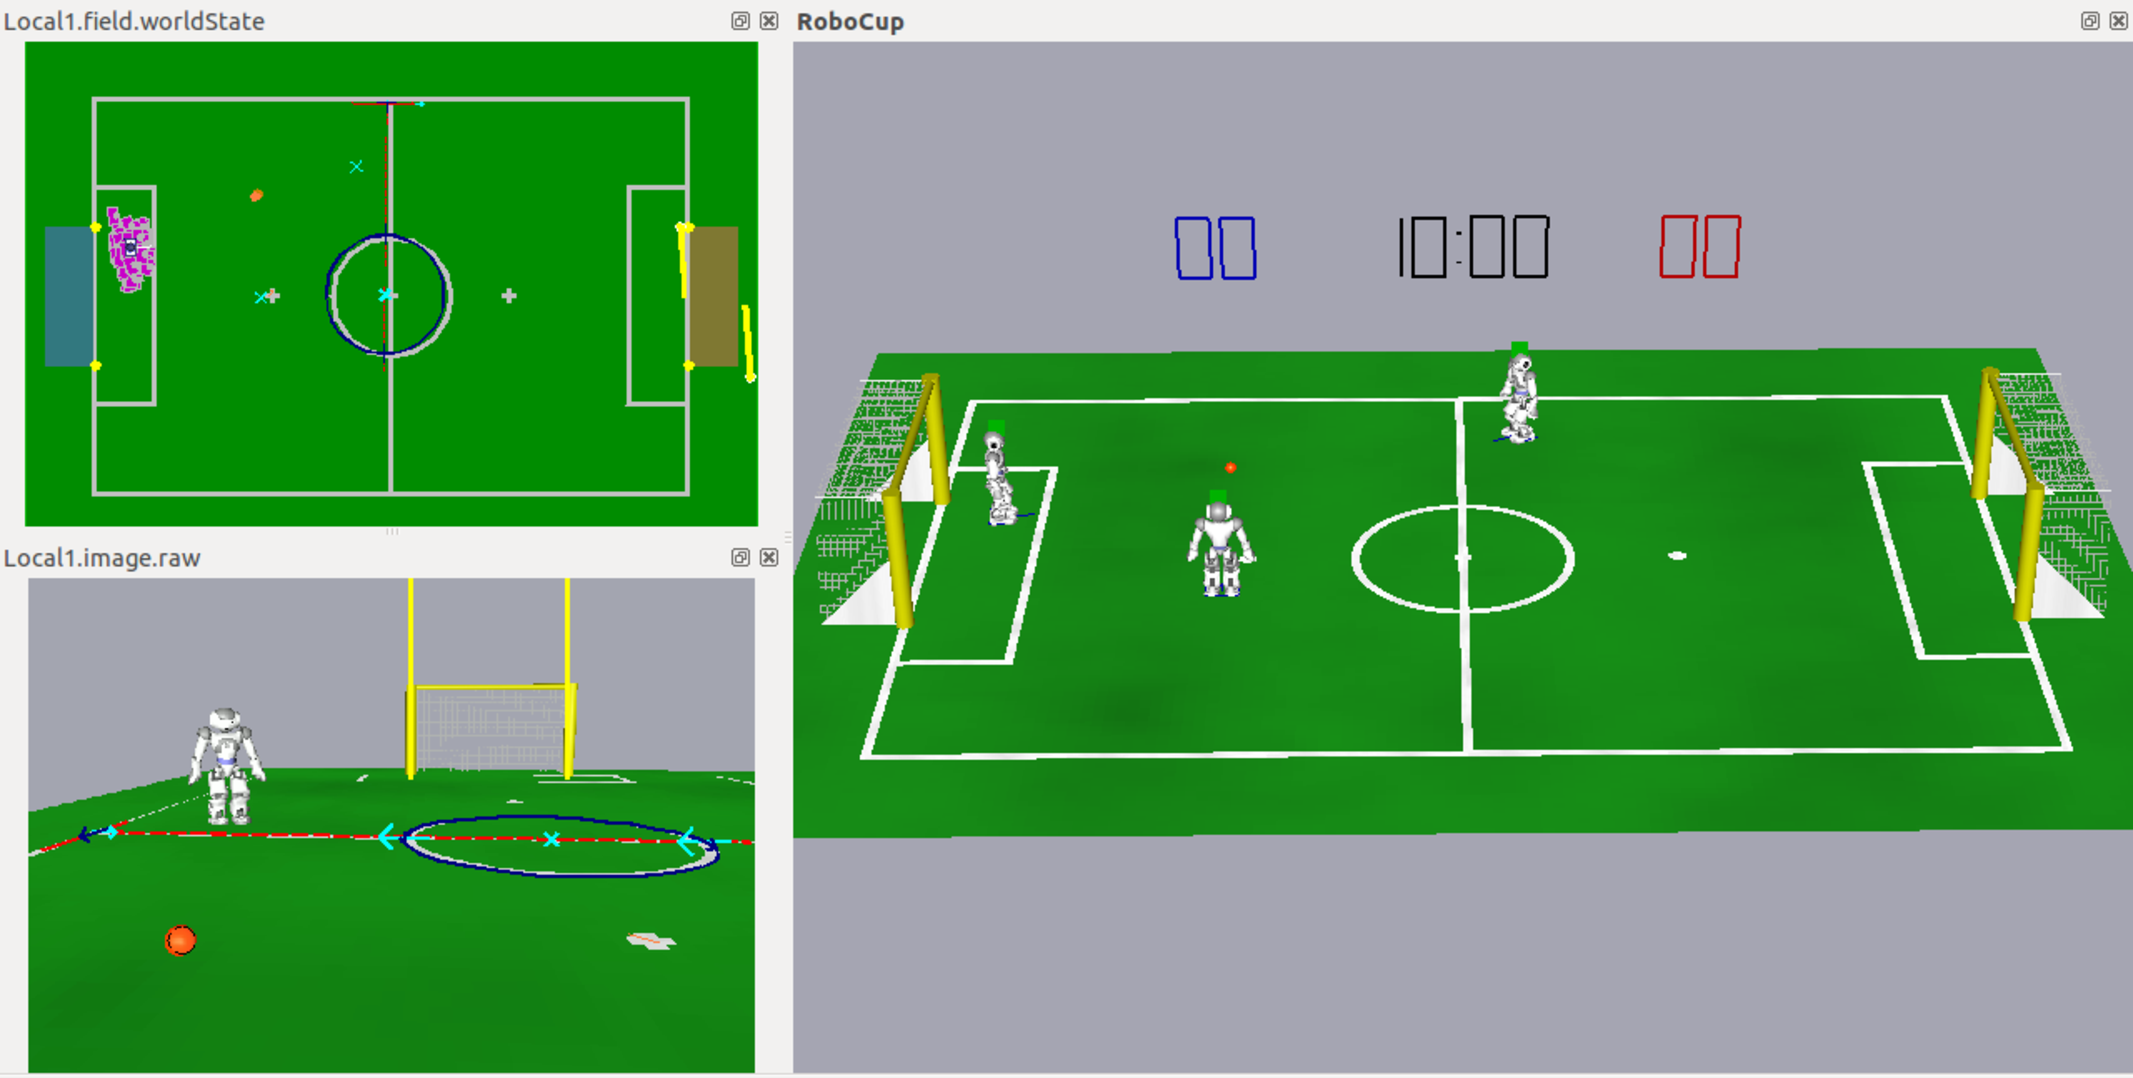
\includegraphics[height=3.1cm]{images/SimRobot}};
			\node at (5.95,0) [draw=black,ultra thick,inner sep=0pt] {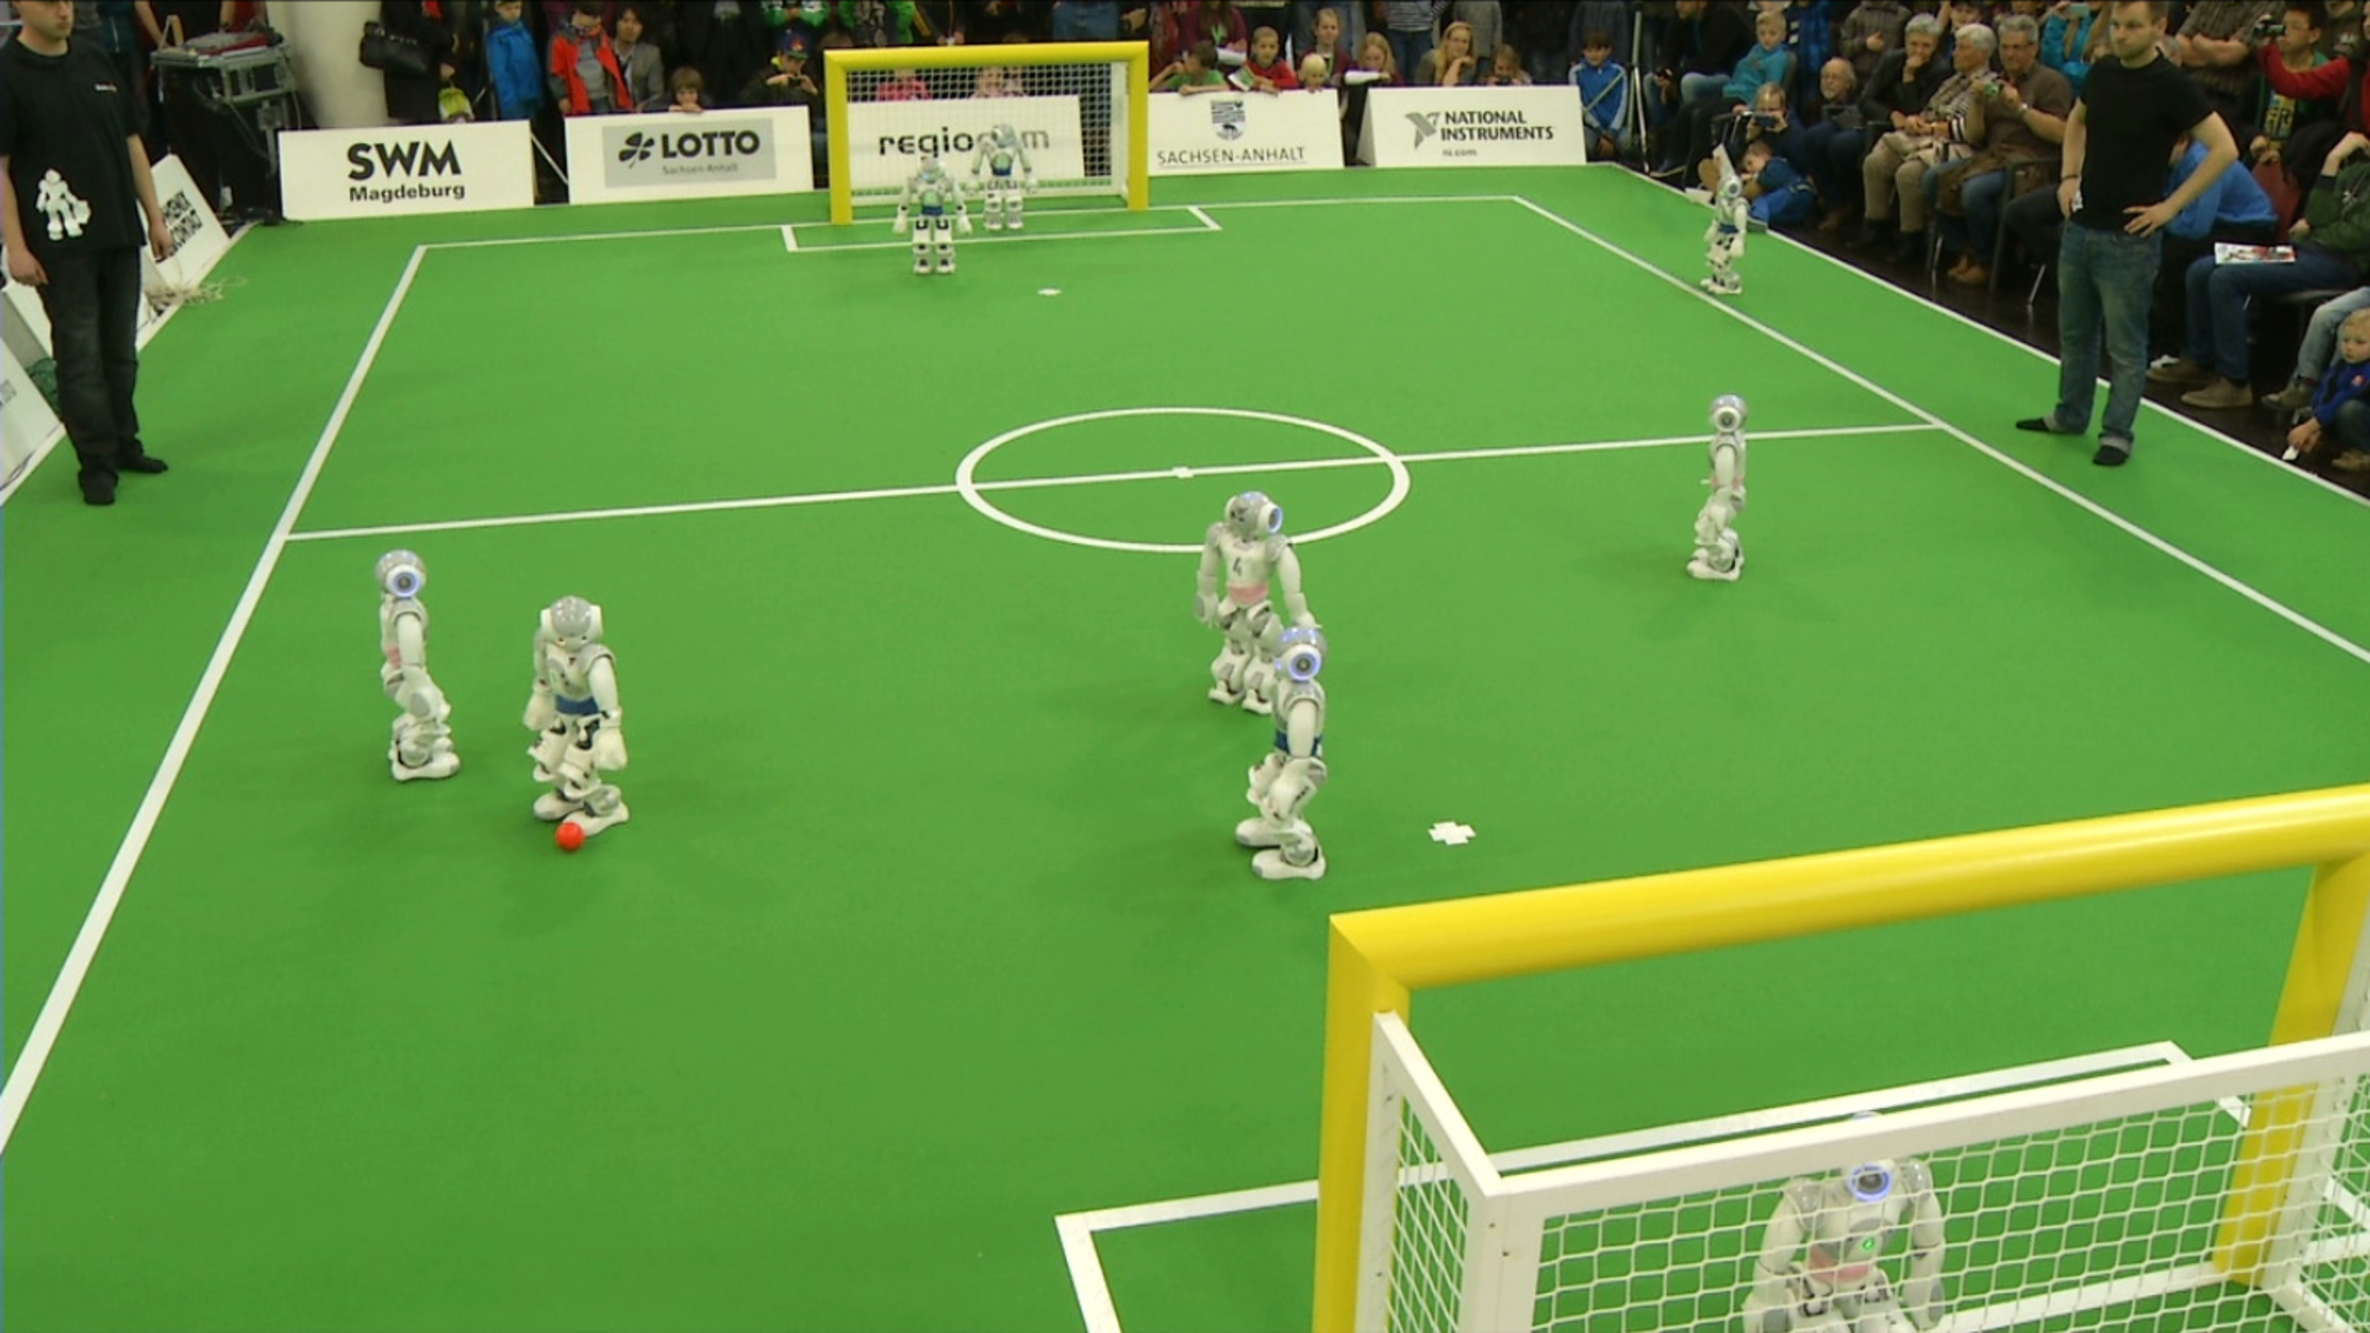
\includegraphics[height=3.1cm]{images/Naos}};
		\end{tikzpicture}
	\end{center}
\end{frame}

\begin{frame}
	\frametitle{Experimental evaluation}
	\framesubtitle{Objective}
	
	\vspace{0.5cm}
	
	Demonstrate, using SimRobot \cite{BHuman11} simulator, the robustness of the PTracking software library by
	adding:
	
	\vspace{0.25cm}
	
	\begin{itemize}
		\item robot localization noise
		\item perception noise
			  \begin{itemize}
			  	\item Increasing the duration of false perceptions
				\item Increasing the number of false perceptions
			  \end{itemize}
	\end{itemize}
	
	\vspace{0.25cm}
	
	We compared the performance, in terms of robustness, of our method with respect to the algorithm developed by Wu
	et al. \cite{Wu08}.
	
	\vspace{1cm}

	\tiny 3. \emph{R\"{o}fer et al.: ``B-human team report and code release 2011''. Technical report, 2011} \\
	\vspace{0.1cm}
	\tiny 4. \emph{Wu et al., ``Boosted Interactively Distributed Particle Filter for automatic multi-object tracking'' in 15th IEEE} \\
	\vspace{-0.18cm}
	\tiny \emph{International Conference on Image Processing, 2008}
\end{frame}

\begin{frame}
	\frametitle{Experimental results}
	\framesubtitle{Nominal situation}
	
	\vspace{0.2cm}
	
	We just introduced the robot localization noise.
	
	\begin{center}
		\begin{tikzpicture}
			\node at (0,0) [draw=white,ultra thick,inner sep=0pt] {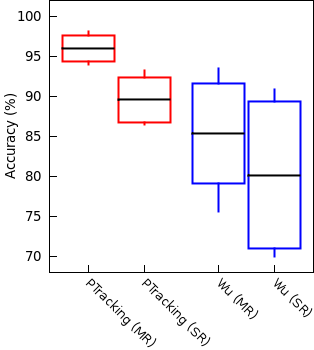
\includegraphics[scale=0.5]{images/Results-NominalSituation.png}};
		\end{tikzpicture}
	\end{center}
\end{frame}

\begin{frame}
	\frametitle{Experimental results}
	\framesubtitle{Increasing the duration of false perceptions}
	
	\vspace{0.3cm}
	
	We introduced both the robot localization noise and we increased the duration of false perceptions.
	
	\vspace{0.1cm}
	
	\begin{center}
		\begin{tikzpicture}
			\node at (0,0) [draw=white,ultra thick,inner sep=0pt] {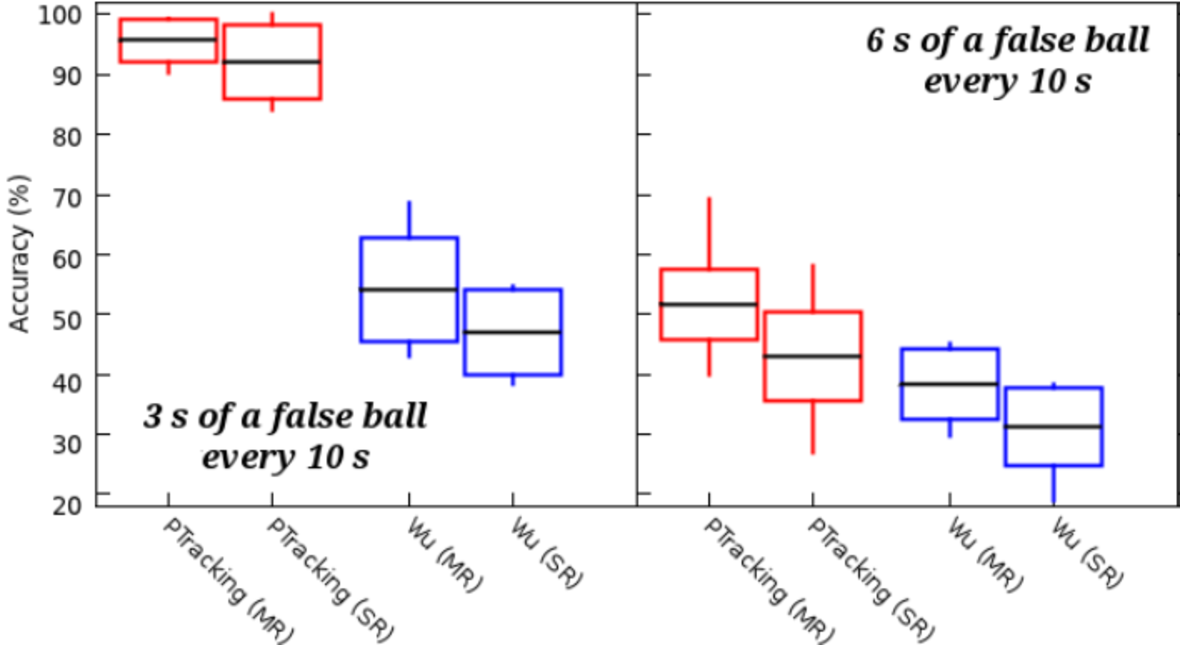
\includegraphics[scale=0.5]{images/Results-PercentageFalseBall}};
		\end{tikzpicture}
	\end{center}
\end{frame}

\begin{frame}
	\frametitle{Experimental results}
	\framesubtitle{Increasing the number of false perceptions}
	
	\vspace{0.3cm}
	
	We introduced both the robot localization noise and we increased the number of false perceptions.
	
	\vspace{0.1cm}
	
	\begin{center}
		\begin{tikzpicture}
			\node at (0,0) [draw=white,ultra thick,inner sep=0pt] {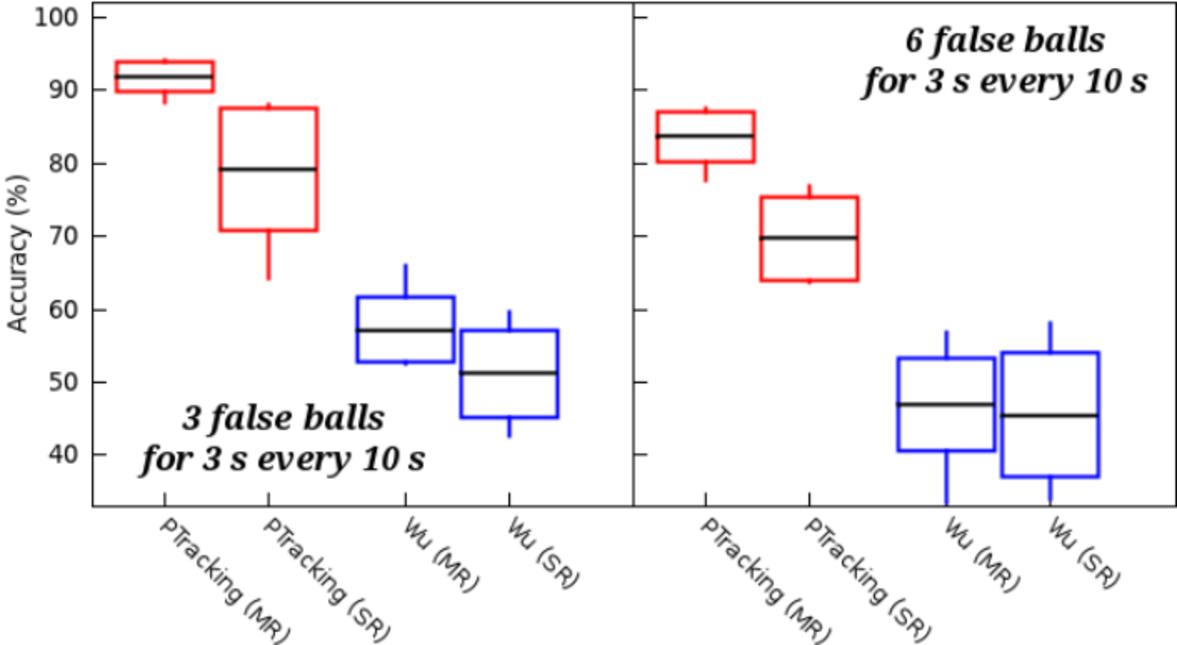
\includegraphics[scale=0.5]{images/Results-FalseBallsAdded}};
		\end{tikzpicture}
	\end{center}
\end{frame}
